% !TeX encoding = UTF-8
\chapter{数值实验}\label{chap6}

\section{经典数值格式收敛阶的验证}
几何Brown运动 $\md X(t) = bX(t) \md t+\sigma X(t)\md B_t$ 的精确解是已知的,且仅与随机项的起点与终点有关,
\[
X_t = X_0 \exp\left[ (b+\frac12\sigma^2)t + \sigma B_t \right]
\]
而不需要知道 $B_t$ 具体的样本轨道形态. 
为了防止 $X_t$ 的值随时间指数增长,选择参数 $(b,\sigma) = (-2,2)$. 
利用该方程验证经典的格式的精度,分别测试误差的期望和方差,结果如下图\ref{fig.6.1}:

\begin{figure}[!htbp]
	\centering 
	\subfigure[误差的期望]{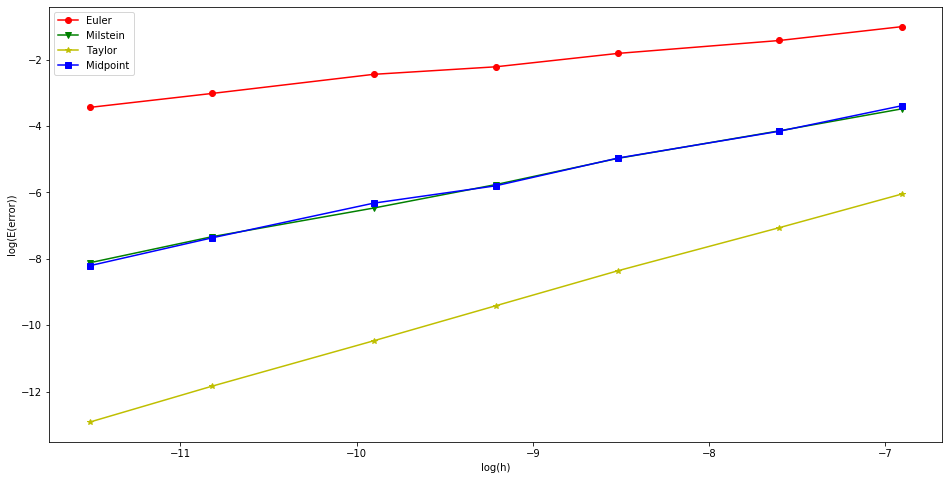
\includegraphics[width=2.95in]{images/6.1.png}}
	\subfigure[误差的方差]{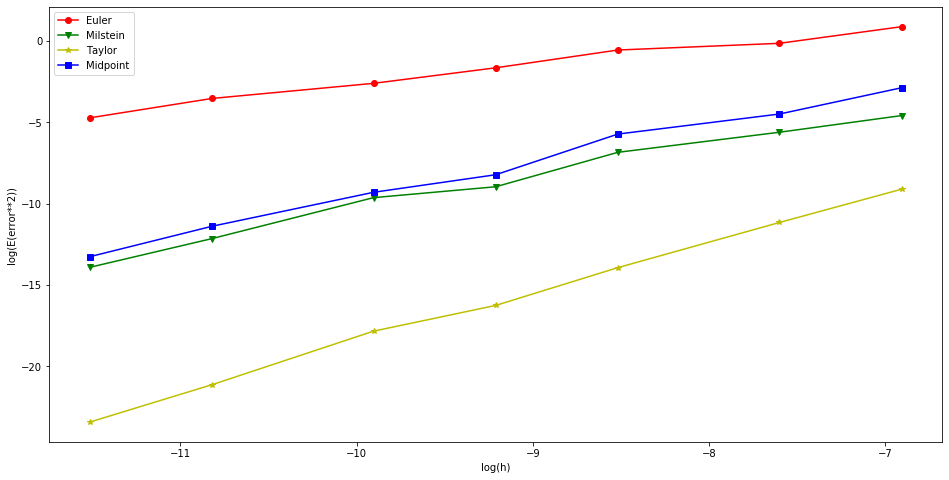
\includegraphics[width=2.95in]{images/6.2.png}}
	\vspace{.2cm}
	\caption{经典数值格式的收敛阶验证}
	\label{fig.6.1}
\end{figure}

测试过程选取了 $10^4$ 条样本轨道进行模拟,步长 $h\in[10^{-5},10^{-3}]$,相较于确定性的微分方程,其计算量大大增加. 根据定理3.1,可以得出 Euler-­Maruyama 格式具有0.5阶误差精度,而Milstein格式和中点公式均有1阶精度,Taylor格式具有最高的1.5阶精度. 中点公式属于隐格式,每次迭代需要求解方程,对于复杂的情况,中点公式的计算效率会受到影响. 

另一方面,估计误差的期望和方差使用 Monte Carlo 的方式,其本身就会存在 $\frac1{\sqrt N}$ 的误差,因此单纯减少步长 $h$ 的方式并不能完整说明数值格式的收敛阶. 对于 Euler-­Maruyama 格式,$N$ 至少与 $\frac1h$同阶,Milstein 格式或中点公式,$N = O(\frac1{h^{2}})$,而 Taylor 格式则是 $O(\frac1{h^{3}})$,因而上述数值实验中存在不可忽略的 Monte Carlo 导致的模拟误差. 

对 Ornstein–Uhlenbeck 方程:$\md X(t) = \mu X_t(t) \md t + \sigma \md B_t $,其真实解为
\[
X_{t}=X_{0} e^{\mu t}+\sigma \int_{0}^{t} e^{\mu(t-s)} \md B_{s}
\]
真实值与积分路径 $B_t$ 有关,而模拟时,数值积分本身就会引入误差,因此无法得到其真实解. 在文献\cite{OUequation}中,构造统计量将方程的参数与该方程的解联系起来. 



\section{稳定解的初值无关性与加速算法的验证}
本节验证4.3节提出的稳定解唯一时的初值无关性并实践加速算法. 考虑测试方程
\begin{equation}\label{example6.2}
\md x  = \left[ \tan(-\frac\pi2x) + \operatorname{sign}(x) \right] \md t + |1-|x||^\alpha \md B_t,\qquad x\in (-1,1).
\end{equation}
文献\cite{Fokker_Planck}指出,当$\alpha < \frac12$时,方程的扩散项不满足 H{\"o}lder 连续性,从而 SDE 的强解的存在唯一性无法保证,但仍然存在概率解. 数值实验考虑边界情况 $\alpha = \frac12$. 
使用Euler-Maruyama格式,对初值无关性的测试结果如下:
\begin{figure}[!htbp]
	\centering 
	\subfigure[$\mu_0 = \delta(\frac13)$]{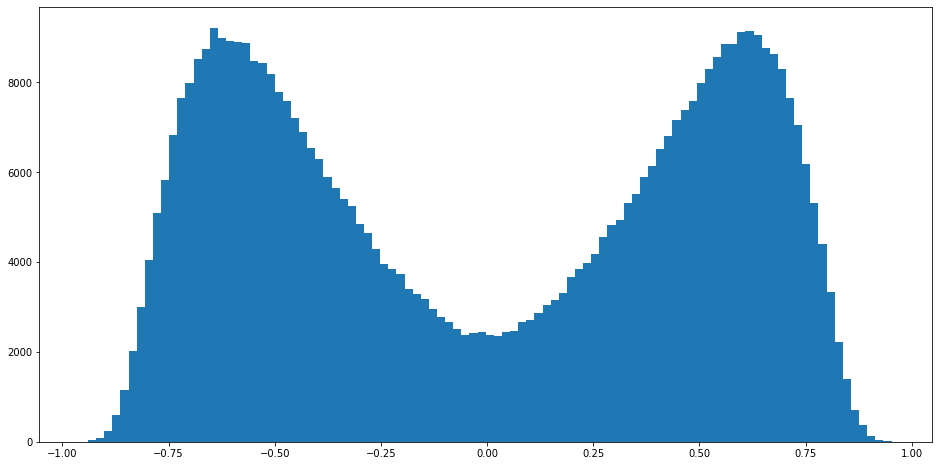
\includegraphics[width=1.95in]{images/6.2/1.png}}
	\subfigure[$\mu_0 = \frac12\delta(-\frac12)+\frac12\delta(\frac12)$]{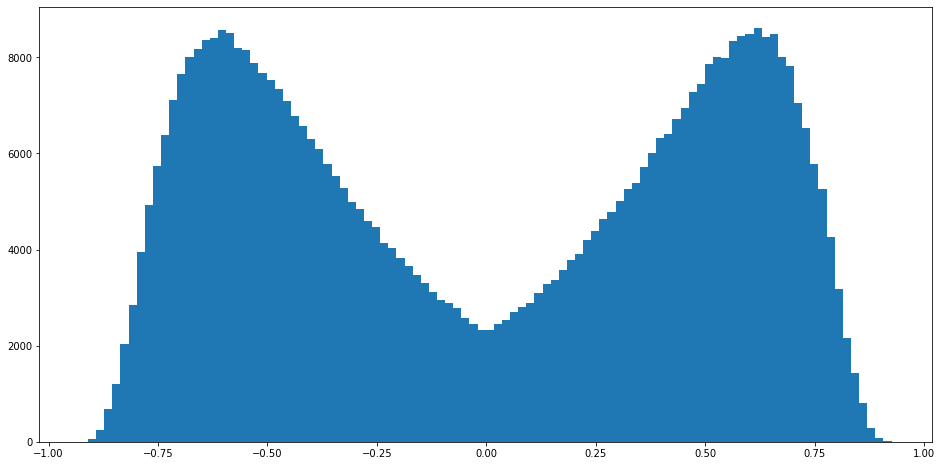
\includegraphics[width=1.95in]{images/6.2/2.png}}
	\subfigure[$\mu_0 = U(-0.999,0.999)$]{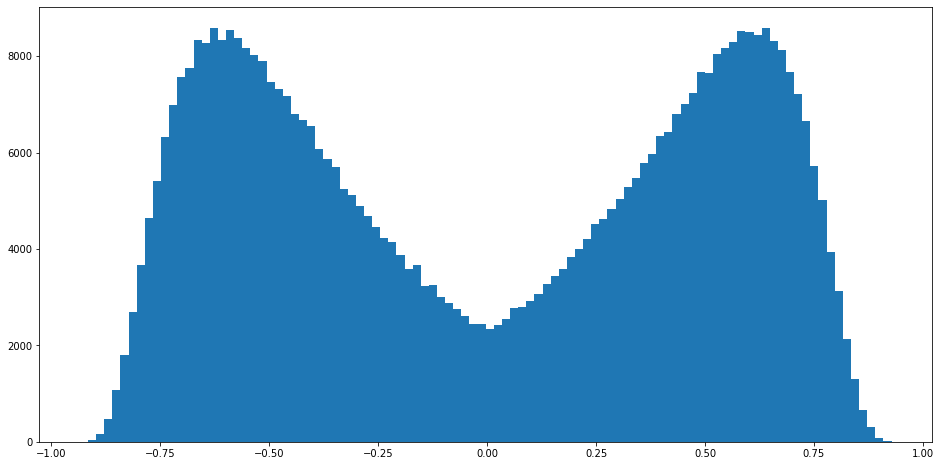
\includegraphics[width=1.95in]{images/6.2/3.png}}
	\vspace{.2cm}
	\caption{稳定解的初值无关性}
	\label{fig.6.2}
\end{figure}

图\ref{fig.6.2}表明,无论初始的分布选择有偏确定值、两点分布或者均匀分布,总是具有相同的稳定解. 注意到稳定解在0和$\pm1$附近的概率较小,而在$\pm0.7$附近拥有最大的概率密度. 结合方程的特点分析:
\begin{enumerate}
	\item[1] 当 $x\approx 0$ 时,方程漂移项较小,但扩散项较大,$x$ 很容易远离 $0$ 附近;
	\item[2] 当 $x\to 1^-$ 或 $x\to (-1)^+$ 时,扩散项很小,但漂移项较大且促使其向 0 移动;
	\item[3] 当 $x\approx 0.7$ 或 $x\approx -0.7$ 时,方程的漂移项和扩散项均不是非常大,$x$ 有更大概率停留,同时接受从0或$\pm1$附近移动过来的点. 
\end{enumerate}
稳定解反映的是随机系统中的粒子出现在各位置的概率值,粒子停留在系统中的时间越长,粒子越容易“遗忘”初始的信息. 

在求解自治随机微分方程时,如果系统存在稳定解,则分析较大的时间 $T$ 对应的概率解 $X_T$ 时,可以直接用稳定解代替. 一方面,随机微分方程计算其数值解时,对于较大的时间 $T$,计算代价会很大. 另一方面,由于稳定解的唯一性、指数收敛率以及加速算法,可以很快得到精度更高的解. 

对加速算法的实践见图\ref{fig.6.3},测试方程仍然取(\ref{example6.2}). 普通方法取步长 $h=10^{-2}$,320次模拟可以演化至 $T=3.20$. 加速算法取初始步长为 $h = \frac12$,每迭代 $\frac1{2h}$ 次后,步长 $h$ 减半,320次迭代可演化至 $T=4.125$,终止时步长 $h=\frac1{512}$. 
\begin{figure}[!htbp]
	\centering 
	\subfigure[$L^1$误差]{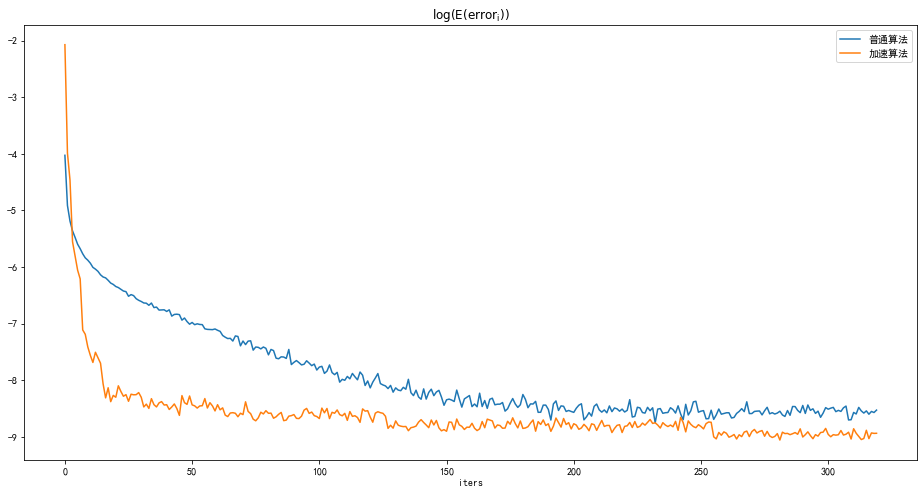
\includegraphics[width=5.95in]{images/6.2-result-1.png}}
	\subfigure[$L^2$误差]{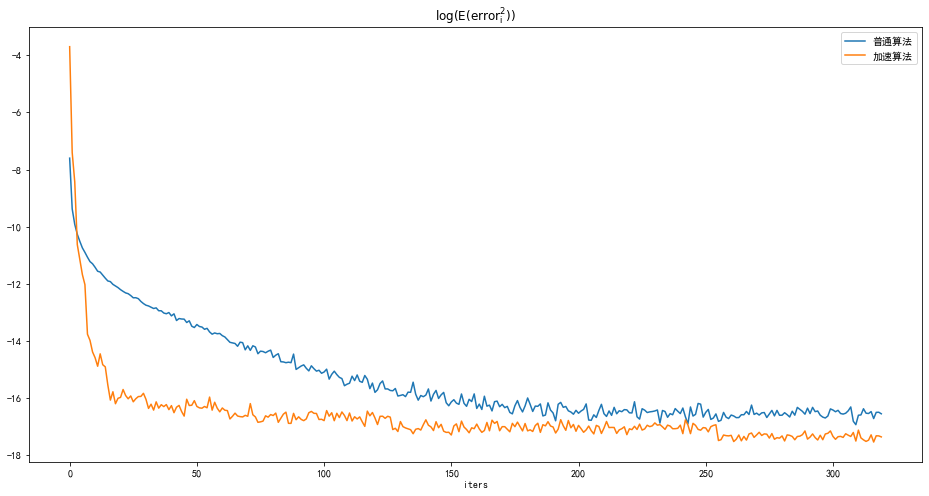
\includegraphics[width=5.95in]{images/6.2-result-2.png}}
	\vspace{.2cm}
	\caption{稳定解加速算法验证}
	\label{fig.6.3}
\end{figure}

由于无法求得稳定解的精确表达式,数值实验考虑相邻两次迭代之间的误差. 与确定性微分方程不同的是,$\md B_t = O(\sqrt{h})$,因此相邻两次迭代的样本轨道之间的误差会远大于 $h$. 假定概率解为 $X^*$,相邻两次的概率解为 $X_n$ 和 $X_{n+1}$,可以近似认为两概率解随机落在 $X^*$ 附近,即 $X_n,X_{n+1} \in Ball(X^*,r),r = \|X_{n+1} - X_n\|$. 


从误差的 $L^1$ 和 $L^2$ 范数的对数可以看出,算法刚开始时,加速算法以很快的速度远离初始分布,并很快到达稳定解附近. 随后随着步长 $h$ 的收缩越来越逼近稳定解. 而普通算法仅能以固定速度偏离初始分布,且时间足够长之后,因步长 $h$ 的限制,精度相较加速算法会显得不足. 






\section{例:二维随机 Kubo oscillator 方程}
本节验证带守恒量的自治随机微分方程的数值解法,对比经典方法和本文提出的算法,数值实验验证了本文提出的算法在保持守恒量方面的优势和数值精度上的变化,并指出本文提出的算法在求解稳定解方面的优势. 

考虑二维的例子:Kubo oscillator 方程:
\begin{equation}\label{eq_Kubo_ito}
\begin{aligned}
& \md x = \left(\frac12 \sigma^2 x(t) - by(t) \right)\md t -\sigma y(t)  \md B_t \\
& \md y =  \left(\frac12 \sigma^2 y(t)+ bx(t) \right)\md t + \sigma x(t)  \md B_t 
\end{aligned}
\end{equation}
其等价的 Stratonovich 型微分方程为
\begin{equation}\label{eq_Kubo_Str}
\begin{aligned}
& \md x = - by(t) \md t - \sigma y(t) \circ \md B_t \\
& \md y =   bx(t) \md t + \sigma x(t) \circ \md B_t 
\end{aligned}
\end{equation}
具有守恒量 $I(x,y) = x^2+y^2$. 有如下的单步数值格式:
\begin{enumerate}
	\item[$\bullet$] 直接差分方法
	\[
	\begin{aligned}
	x_{n+1} = x_n - by_nh - \sigma y_n \Delta_B \\
	y_{n+1} = y_n + bx_nh + \sigma x_n \Delta_B  
	\end{aligned}
	\]
	\item[$\bullet$] Euler-Maruyama 格式(0.5阶精度)
	\[
	\begin{aligned}
	x_{n+1} = x_n + (\frac12\sigma^2x_n-by_n)h - \sigma y_n \Delta_B \\
	y_{n+1} = y_n + (\frac12\sigma^2y_n+bx_n)h + \sigma x_n \Delta_B  
	\end{aligned}
	\]
	\item[$\bullet$] Milstein 格式(1阶精度)
	\[
	\begin{aligned}
	x_{n+1} = x_n + (\frac12\sigma^2x_n-by_n)h - \sigma y_n \Delta_B -\frac12\sigma^2x_n \Delta_B^2 \\
	y_{n+1} = y_n + (\frac12\sigma^2y_n+bx_n)h + \sigma x_n \Delta_B -\frac12\sigma^2y_n \Delta_B^2 
	\end{aligned}
	\]
	\item[$\bullet$] Taylor 格式(1.5阶精度)
	\[
	\begin{aligned}
	x_{n+1} = x_n &+ (\frac12\sigma^2x_n-by_n)h - \sigma y_n \Delta_B 
					 -\frac12\sigma^2x_n \Delta_B^2 
					+\frac16\sigma^3y_n(\Delta_B^3-3h\Delta_B)\\
				  &-(\frac12\sigma^3y_n+\sigma bx_n)h\Delta_B
				  +(\frac18\sigma^4x_n-\frac12\sigma^2by_n-\frac12b^2x_n)h^2\\
	y_{n+1} = y_n &+ (\frac12\sigma^2y_n+bx_n)h + \sigma x_n \Delta_B
					 -\frac12\sigma^2y_n \Delta_B^2 
					 -\frac16\sigma^3x_n(\Delta_B^3-3h\Delta_B)\\
				  &+(\frac12\sigma^3x_n-\sigma by_n)h\Delta_B
				  +(\frac18\sigma^4y_n+\frac12\sigma^2bx_n-\frac12b^2y_n)h^2
	\end{aligned}
	\]
\end{enumerate}
注意到直接差分方法并不等同于 Euler-Maruyama 格式,对于随机微分方程,二次变差项不能忽略. 
现考虑其守恒量,根据5.1节的格式(\ref{scheme_discrete_1})和(\ref{scheme_discrete_2}),推导保守恒量的数值格式. 取 
\[
\begin{aligned}
&S(x) =  \frac{f(x) \nabla I(x)^T - \nabla I(x) f(x)^T}{|\nabla I(x)|^2} \\
&T(x) =  \frac{g(x) \nabla I(x)^T - \nabla I(x) g(x)^T}{|\nabla I(x)|^2} 
\end{aligned}
\]
得
\[
S = \begin{pmatrix} 0&-b\\b&0\end{pmatrix}, \qquad
T = \begin{pmatrix} 0&-\sigma\\\sigma&0\end{pmatrix}
\]
因此二维 Kubo oscillator 方程的 SG 格式为:
\begin{equation}
	\md \begin{pmatrix} x(t) \\ y(t)	\end{pmatrix} = \frac12
	\begin{pmatrix} 0&-1 \\  1&0	\end{pmatrix} 
	\begin{pmatrix} I_x \\ I_y	\end{pmatrix} (b \md t + \sigma \md B_t).
\end{equation}
因 $S$ 为常系数矩阵,从而离散梯度格式(\ref{scheme_discrete_1})和(\ref{scheme_discrete_2}一致,为
\begin{equation}\label{scheme-SG}
\begin{aligned}
	&x_{n+1} = x_n - \frac b2(y_n+y_{n+1})h -\frac \sigma 2 (y_n+y_{n+1}) \Delta_B\\
	&y_{n+1} = y_n + \frac b2(x_n+x_{n+1})h +\frac \sigma 2 (x_n+x_{n+1}) \Delta_B
\end{aligned}
\end{equation}
上述格式为隐格式,但可以显式求解出来. 

考虑到该随机微分方程不存在精确解的表示式,使用Taylor方法的计算结果作为真值. 通过数值实验也验证了经典数值格式的误差精度,并说明格式(\ref{scheme-SG})同样具有一阶整体精度.

图\ref{fig.6.4}说明离散梯度格式具有1阶整体精度. 图\ref{fig.6.5}说明步长 $h$ 越小,守恒量偏离初始值的就越少,但除了离散梯度格式,其余算法均固定向某一个方向偏移,而离散梯度格式在所有的样本轨道上均能保持守恒量 $x^2+y^2$ 始终为1.图\ref{fig.6.6}取步长 $h=0.05$,数值结果说明随着时间增长,守恒量的偏移方向始终是一致的,因而时间越长,结果越不可取. 除了保持守恒量的离散梯度格式外,其余算法均呈现精度越高,守恒量误差也越少,这也是合理的. 

\begin{figure}[!htbp]
	\centering 
	\subfigure[$L^1$误差]{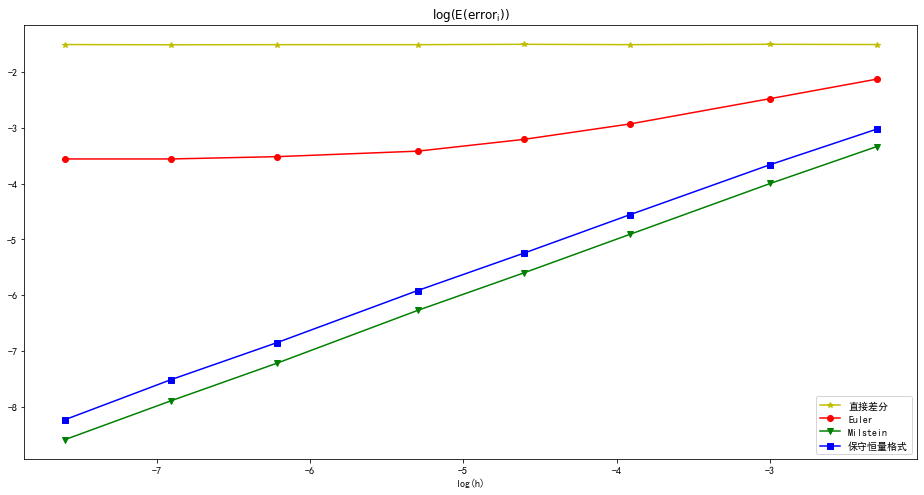
\includegraphics[width=2.95in]{images/6.3/1.png}}
	\subfigure[$L^2$误差]{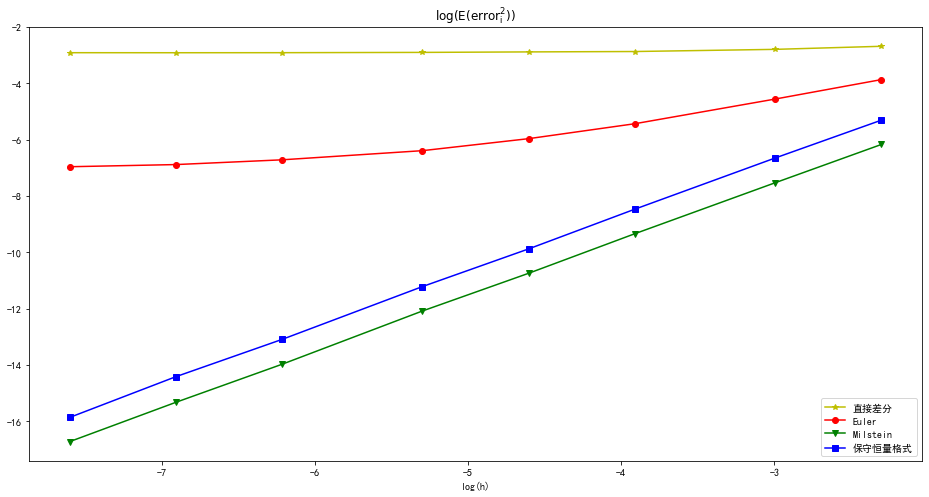
\includegraphics[width=2.95in]{images/6.3/2.png}}
	\vspace{.2cm}
	\caption{二维 Kubo oscillator 方程数值格式的误差}
	\label{fig.6.4}
\end{figure}

\begin{figure}[!htbp]
	\centering 
	\subfigure[守恒量的均值]{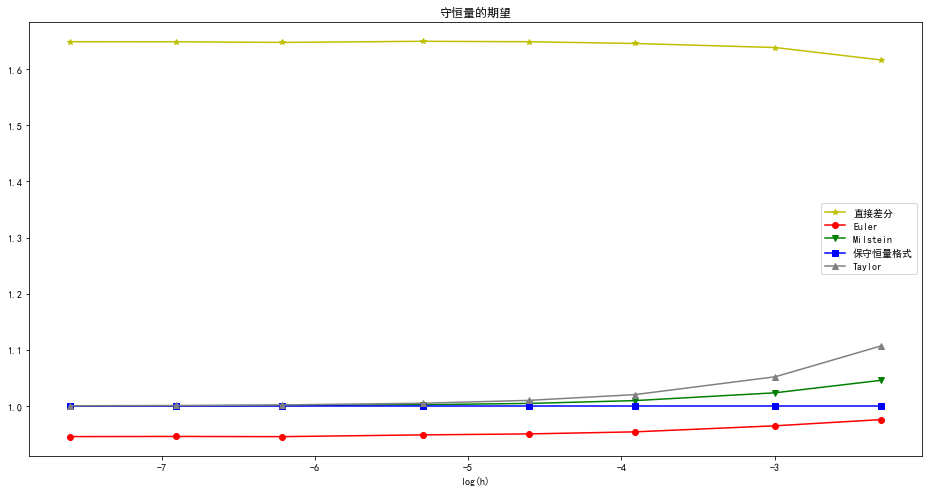
\includegraphics[width=2.95in]{images/6.3/3.png}}
	\subfigure[守恒量的方差]{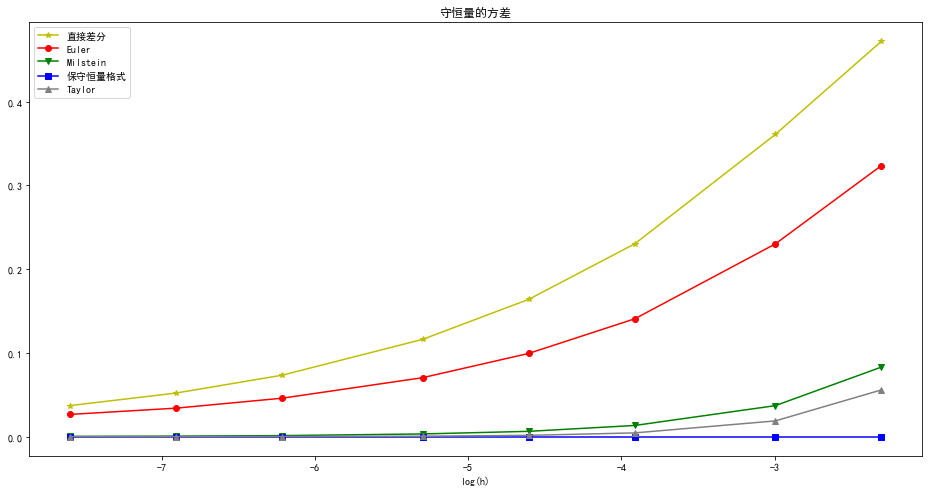
\includegraphics[width=2.95in]{images/6.3/4.png}}
	\vspace{.2cm}
	\caption{二维 Kubo oscillator 方程数值格式的守恒量}
	\label{fig.6.5}
\end{figure}




\begin{figure}[!htbp]
	\centering 
	\subfigure[守恒量的均值]{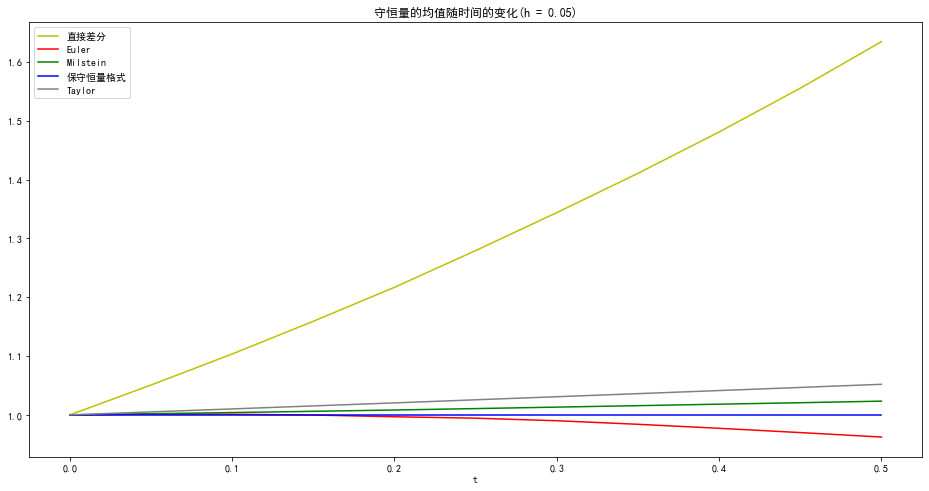
\includegraphics[width=2.95in]{images/6.3/5.png}}
	\subfigure[守恒量的方差]{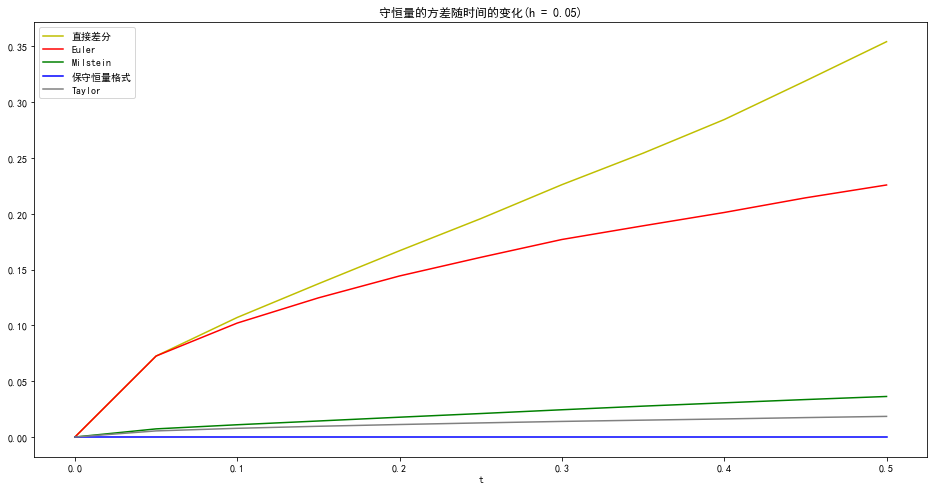
\includegraphics[width=2.95in]{images/6.3/6.png}}
	\vspace{.2cm}
	\caption{二维 Kubo oscillator 方程守恒量随时间的变化}
	\label{fig.6.6}
\end{figure}



通过投射的思想,可以直接将单步法改造成对应的投射方法. 考虑到该守恒量对应的流形是单位圆周,因此可以直接选择投射到距离最近的点上. 考虑初值 $(x,y) = (1,0)$,步长 $h= 0.01$,对5000条样本轨道进行模拟,Euler格式、Milstein格式、EulerP格式结果如下:
\begin{figure}[!htbp]
	\centering 
	\subfigure[T=0.5]{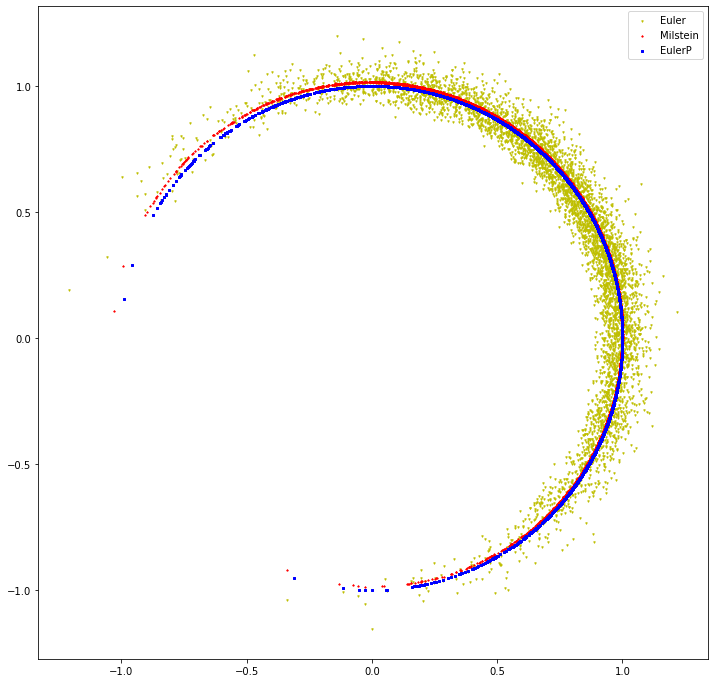
\includegraphics[width=1.95in]{images/6.3/7(T=0.5).png}}
	%\subfigure[T=1.0]{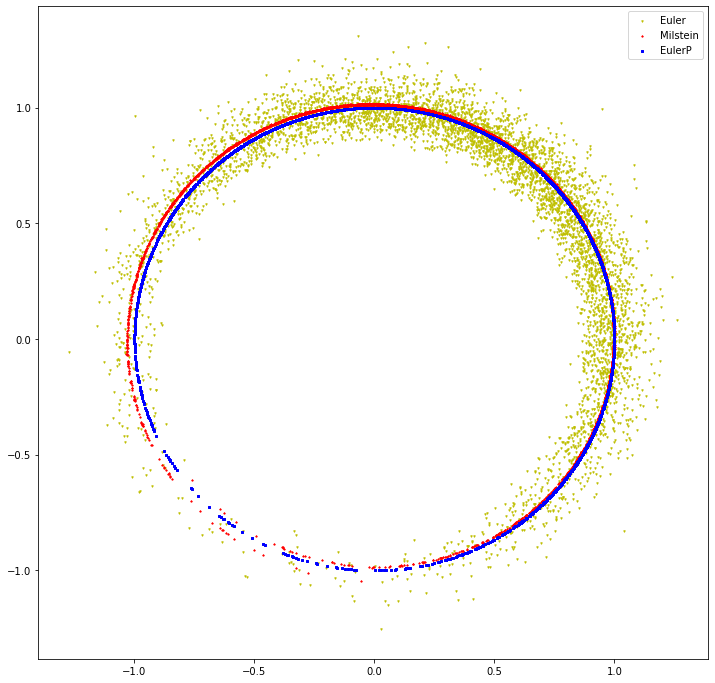
\includegraphics[width=1.95in]{images/6.3/8(T=1).png}}
	\subfigure[T=5.0]{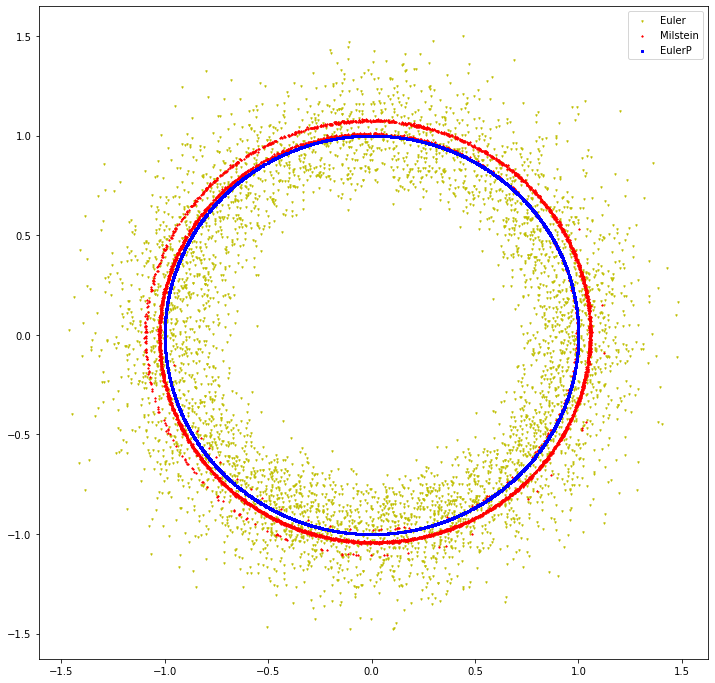
\includegraphics[width=1.95in]{images/6.3/9(T=5).png}}
	\subfigure[T=20.0]{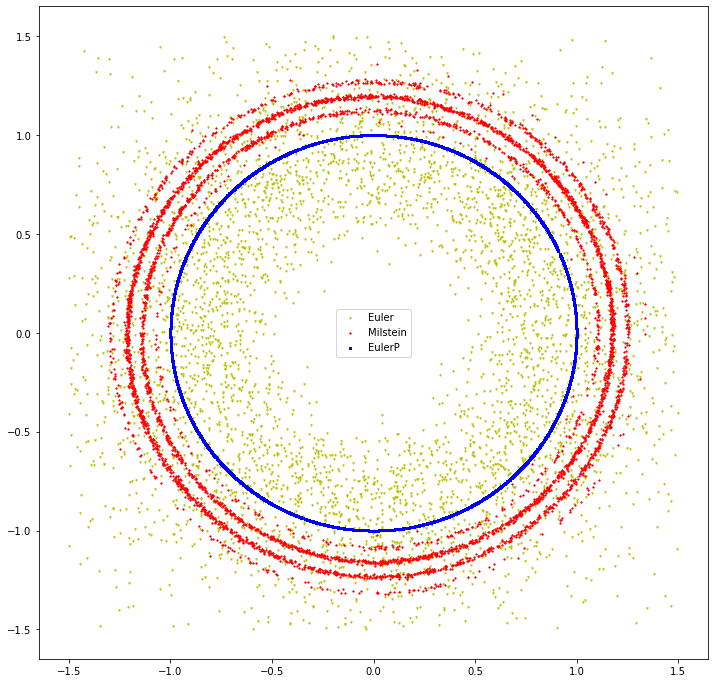
\includegraphics[width=1.95in]{images/6.3/10(T=20).png}}
	\vspace{.2cm}
	\caption{Euler,Milstein,EulerP格式}
	\label{fig.6.7}
\end{figure}

模拟结果与图\ref{fig.6.6}一致,Euler 格式守恒量的方差要大得多,且守恒量均值略小于初始守恒量,而 Milstein 格式守恒量方差较小,均值略大于初始守恒量. 进一步分析 EulerP、MilsteinP 格式的收敛阶,由图\ref{fig.6.8}可以看出 EulerP、MilsteinP 的精度均比对应的单步方法 Euler格式、Milstein格式高. 
\begin{figure}[!htbp]
	\centering 
	\subfigure[守恒量的均值]{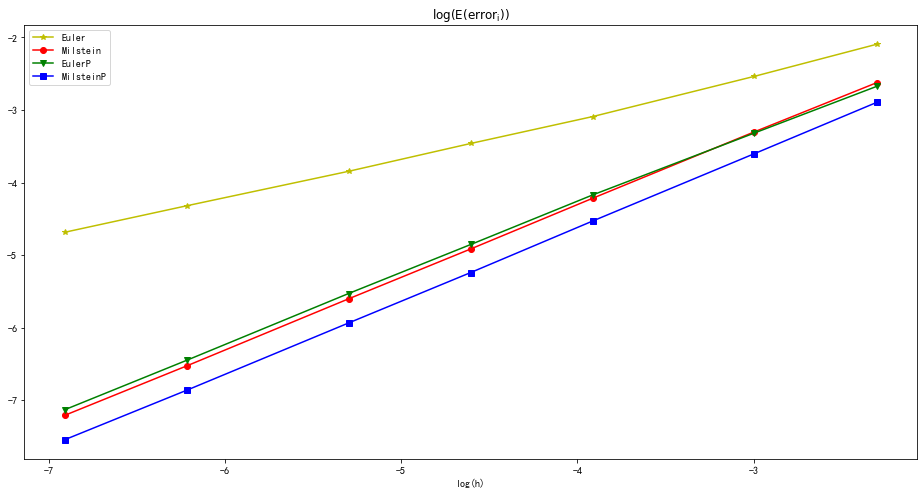
\includegraphics[width=2.95in]{images/6.3/11.png}}
	\subfigure[守恒量的方差]{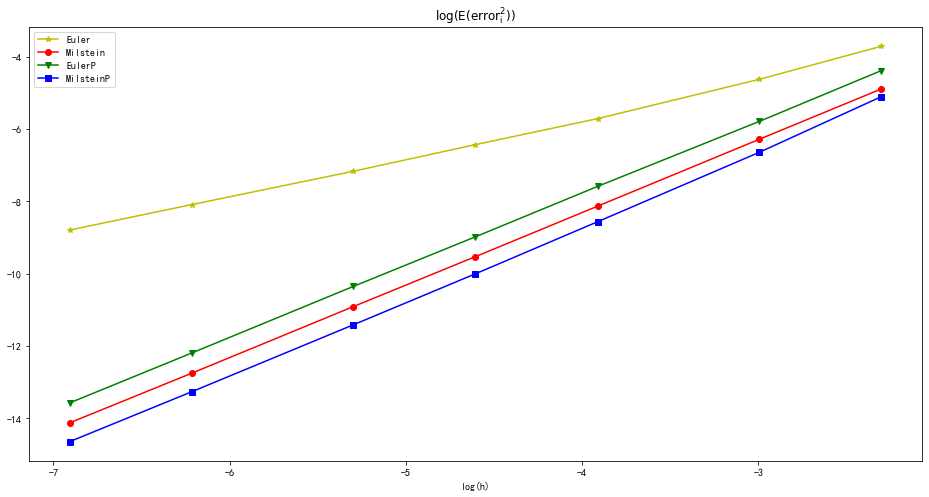
\includegraphics[width=2.95in]{images/6.3/12.png}}
	\vspace{.2cm}
	\caption{二维 Kubo oscillator 方程守恒量随时间的变化}
	\label{fig.6.8}
\end{figure}


使用本文提出的加速算法演化(\ref{eq_Kubo_ito})的稳定解,由图\ref{fig.6.9}可以看出,该随机系统达到稳定状态时,粒子在 $\pm 1$ 附近出现的概率更大,并且 $X,Y$ 的稳定解几乎是一致的. 但值得注意的是,这边的数值格式必须要保持守恒量不变,否则不满足 $(x,y) \in [-1,1]\times [-1,1]$ 的条件,因而绝对不可能得到图\ref{fig.6.9}的稳定结果. 

\

\begin{figure}[!htbp]
	\centering 
	\subfigure{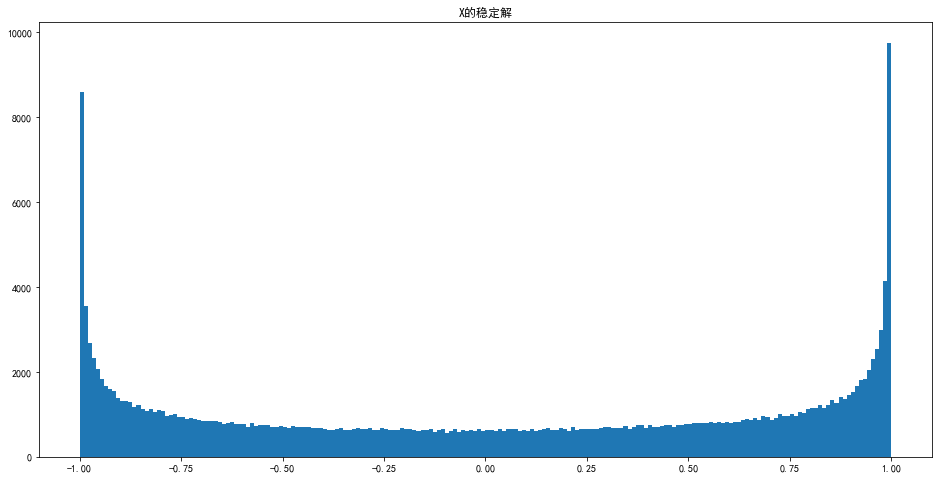
\includegraphics[width=2.95in]{images/Kubo/kubo-x.png}}
	\subfigure{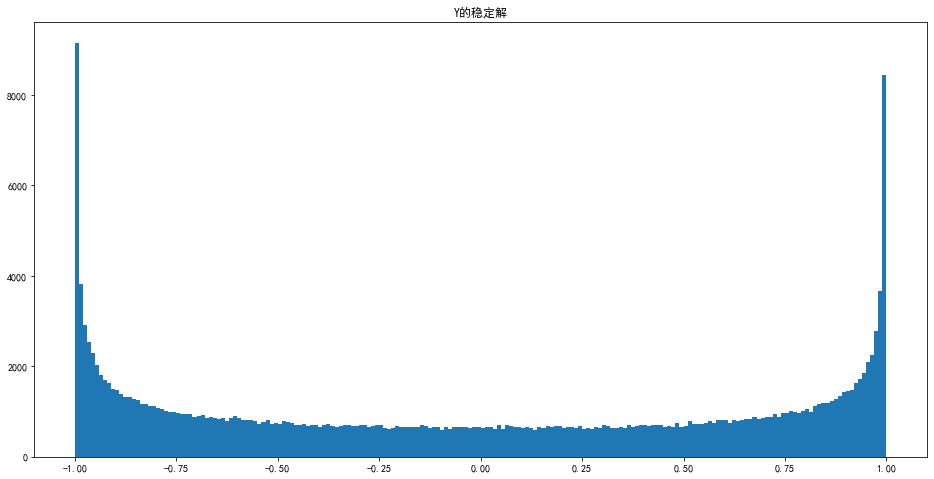
\includegraphics[width=2.95in]{images/Kubo/kubo-y.png}}
	\vspace{.2cm}
	\caption{二维 Kubo oscillator 方程的稳定解}
	\label{fig.6.9}
\end{figure}




对问题(\ref{eq_Kubo_Str})做坐标旋转,得
\[
\md 
\begin{pmatrix} x\\y\end{pmatrix}
\begin{pmatrix} \cos \theta & \sin \theta \\ -\sin \theta & \cos \theta \end{pmatrix}
= 
\begin{pmatrix} 0&-1 \\  1&0	\end{pmatrix} 
\begin{pmatrix} x \\ y	\end{pmatrix} 
\begin{pmatrix} \cos \theta & \sin \theta \\ -\sin \theta & \cos \theta \end{pmatrix}
(b \md t + \sigma \md B_t).
\]
与坐标旋转之前具有一致的微分形式,故 $(x,y)$ 具有旋转对称性. 因此稳定解 $(x,y)$ 是守恒量对应的流形上的均匀分布,则概率密度函数为:
\[
P (x=a) = \frac{1}{\pi\sqrt{1-a^2}},\qquad P(y=b) = \frac{1}{\pi\sqrt{1-b^2}}.
\]
其在区间 $[t_n,t_{n+1}]$ 上的概率值为 $\frac1\pi\left(\operatorname{arcsin}(t_{n+1}) - \operatorname{arcsin}{(t_{n})}\right)$. 其概率分布柱状图如下. 
\begin{figure}[!htbp]
	\centering 
	\subfigure{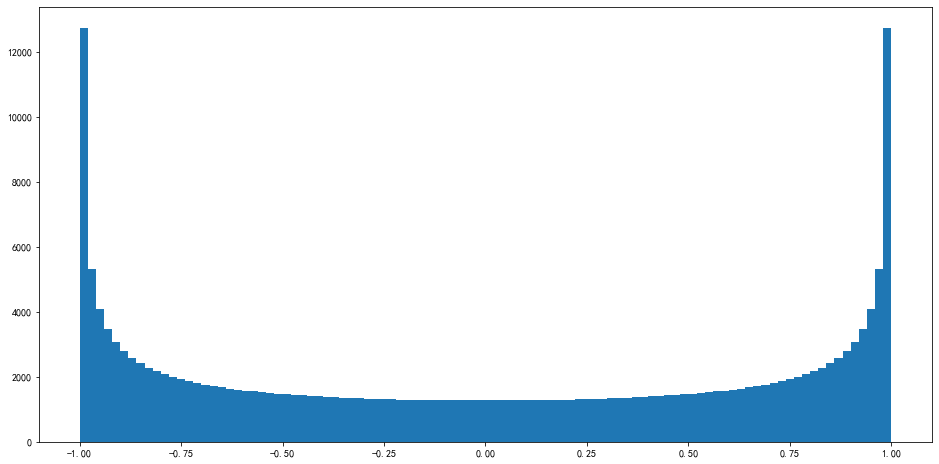
\includegraphics[width=2.95in]{images/Kubo/thoery_hist.png}}
	\vspace{.2cm}
	\label{fig.6.10}
\end{figure}
与模拟的结果也是一致的. 因此在求解该自治随机微分方程时,稳定解为圆周上的均匀分布,且不论初值情况如何,对 $T>1$ 的情况,可以直接用稳定解代替数值格式得到的解. 
即对演化时间足够长的情况,概率解为
\begin{equation}
\mu_{_T}(x,y) \approx
\left\{
\begin{aligned}
&\frac1{2\pi \sqrt{x_0^2+y_0^2}}, \qquad  & \rm{if}\quad x^2+y^2=x_0^2+y_0^2,\\
& 0,\qquad  & \rm{if}\quad x^2+y^2\neq x_0^2+y_0^2 .
\end{aligned}
\right.
\end{equation}

在离散操作过程中,不考虑守恒量时无法注意到该方程存在稳定解. 但使用保持守恒量的数值格式,则很容易得到该方程的稳定解. 这说明对于演化过程较长的情况,引入守恒量对概率解精度的提升是非常巨大的. 由稳定解的唯一性和指数收敛的特性,使用保守恒量的数值格式计算得到的稳定解的误差是有界的. 
并且可以做出如下猜想:当自治随机微分方程存在守恒量,且守恒量对应的流形的测度有限时,只要存在概率解,就必定存在唯一的稳定解. 


\section{例:三维随机 Lotka Volterra 方程}
本节通过高维的例子验证间接离散梯度算法的有效性. 考虑三维随机 Lotka Volterra 方程,
\begin{equation}\label{eq6.7}
\md 
\begin{pmatrix} x \\y \\z \end{pmatrix}
=
\begin{pmatrix}x(z-y) \\y(x-z) \\z(y-x)\end{pmatrix} \md t
+
\begin{pmatrix} x(z-y) \\y(x-z) \\z(y-x)\end{pmatrix} \circ \md B_t
\end{equation}
具有守恒量 $I(x,y,z) = x+y+z$. 
此处为了格式的简洁,不考虑 \ito 意义下的微分方程. 
由于该方程同样不存在精确解的表达式,且 Taylor 格式存在不可积分项,无法写出,因此本节的参照格式为 Milstein 格式. 计算 $\frac12 \frac {\partial g(X)}{\partial X} g(X)$,得其格式:
\[
\begin{aligned}
&x_{n+1}=x_{n}+x_{n}\left(z_{n}-y_{n}\right)(h+\Delta _B)
	+\frac{1}{2}\left(x_{n}\left(y_{n}^{2}+z_{n}^{2}-x_{n}\left(y_{n}+z_{n}\right)\right)\right) \Delta_B^2\\
&y_{n+1}=y_{n}+y_{n}\left(x_{n}-z_{n}\right)(h+\Delta _B)
	+\frac{1}{2}\left(y_{n}\left(z_{n}^{2}+x_{n}^{2}-y_{n}\left(x_{n}+z_{n}\right)\right)\right) \Delta_B^2\\
&z_{n+1}=z_{n}+z_{n}\left(y_{n}-x_{n}\right)(h+\Delta _B)
	+\frac{1}{2}\left(z_{n}\left(x_{n}^{2}+y_{n}^{2}-z_{n}\left(x_{n}+y_{n}\right)\right)\right)\Delta_B^2
\end{aligned}
\]
再分析其 SG形式为:
\begin{equation}\label{eq6.9}
\md\left(\begin{array}{l}
	x \\
	y \\
	z
\end{array}\right)=\left(\begin{array}{ccc}
	0 & -\frac{2 x y-x z-y z}{3} & -\frac{x y+y z-2 x z}{3} \\
	\frac{2 x y-x z-y z}{3} & 0 & -\frac{2 y z-x y-x z}{3} \\
	\frac{x y+y z-2 x z}{3} & \frac{2 y z-x y-x z}{3} & 0
\end{array}\right)\left(\begin{array}{l}
	1 \\
	1 \\
	1
\end{array}\right)(\md t + \circ  \md B_t)
\end{equation}
将其拆解为如下三个子系统
\begin{align*}
\left\{
\begin{array}{l}
\md\left(\begin{array}{l}
x \\
y
\end{array}\right)=\left(\begin{array}{cc}
0 & -\frac{2 x y-x z-y z}{3} \\
\frac{2 x y-x z-y z}{3} & 0
\end{array}\right)\left(\begin{array}{l}
1 \\
1
\end{array}\right)(\md t + \circ \md B_t) \\
\md z=0
\end{array}       
\right.        \tag{\ref{eq6.9}{.a}}\\
\left\{\begin{array}{l}
\md\left(\begin{array}{c}
x \\
z
\end{array}\right)=\left(\begin{array}{cc}
0 & -\frac{x y+y z-2 x z}{3} \\
\frac{x y+y z-2 x z}{3} & 0
\end{array}\right)\left(\begin{array}{l}
1 \\
1
\end{array}\right)(\md t + \circ \md B_t) \\
\md y=0
\end{array}
\right.        \tag{\ref{eq6.9}{.b}}\\
\left\{
\begin{array}{l}
\md\left(\begin{array}{l}
y \\
z
\end{array}\right)=\left(\begin{array}{cc}
0 & -\frac{2 y z-x y-x z}{3} \\
\frac{2 y z-x y-x z}{3} & 0
\end{array}\right)\left(\begin{array}{l}
1 \\
1
\end{array}\right)(\md t + \circ \md B_t) \\
\md x=0
\end{array}     
\right.        \tag{\ref{eq6.9}{.c}}
\end{align*}
使用隐格式 (\ref{scheme_discrete_1})或(\ref{scheme_discrete_2})处理上述三个子系统,均不能得到显式表达式. 使用非线性求解器求解隐格式,效率则会下降很多,数值实验表明,该格式尽管可以保证误差精度,但并不能得到一个稳定解. 这是因为方程(\ref{eq6.7})还存在另一个守恒量 $I_2(x,y,z) = xyz$,而SG形式不能处理带多个守恒量的问题. 投射方式采用到守恒量流形的 $L^2$ 距离最小的方式选取. 使用拉格朗日乘子法,得拉格朗日函数:
\[
L(x,y,z,\lambda_1,\lambda_2) = \frac12\left[
(x-x^*)^2+(y-y^*)^2+(z-z^*)^2
\right]
+\lambda_1(x+y+z-I) +  \lambda_2(xyz-I_2).
\]
数值实验很好的验证了该数值格式的精度和对守恒量保持的特性. 
\begin{figure}[!htbp]
	\centering 
	\subfigure{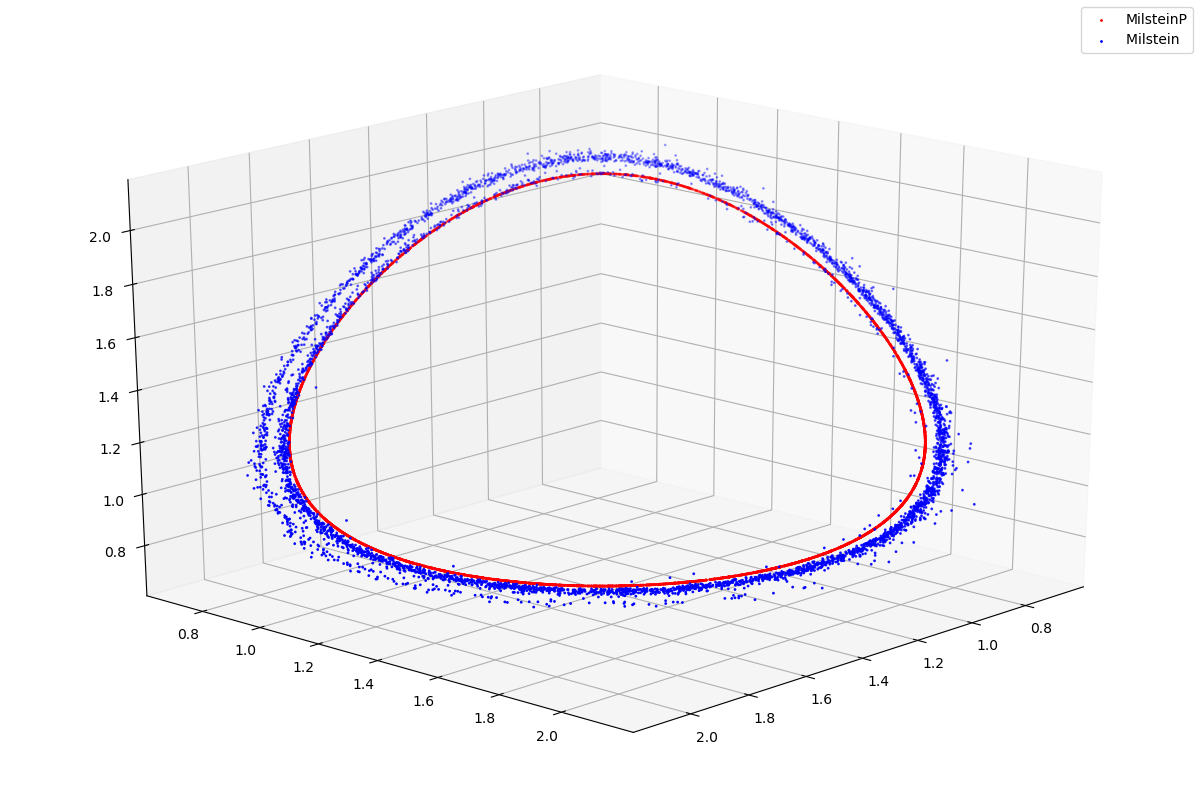
\includegraphics[width=5.95in]{images/Lotka/Figure_2.png}}
	\vspace{.2cm}
	\caption{三维随机 Lotka Volterra 方程的解}
	\label{fig.6.11}
\end{figure}
数值模拟得到 $I=4,I_2=2$ 时方程的稳定解,比对6.3节二维实验的结果,可以近似认为稳定解是守恒量对应的流形上的均匀分布. 
\begin{figure}[!htbp]
	\centering 
	\subfigure[X的稳定解]{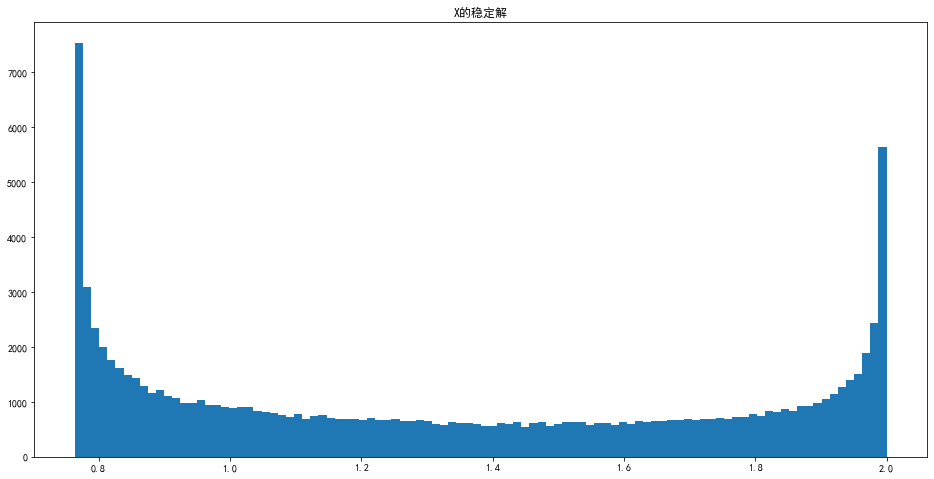
\includegraphics[width=1.95in]{images/Lotka/x.png}}
	\subfigure[Y的稳定解]{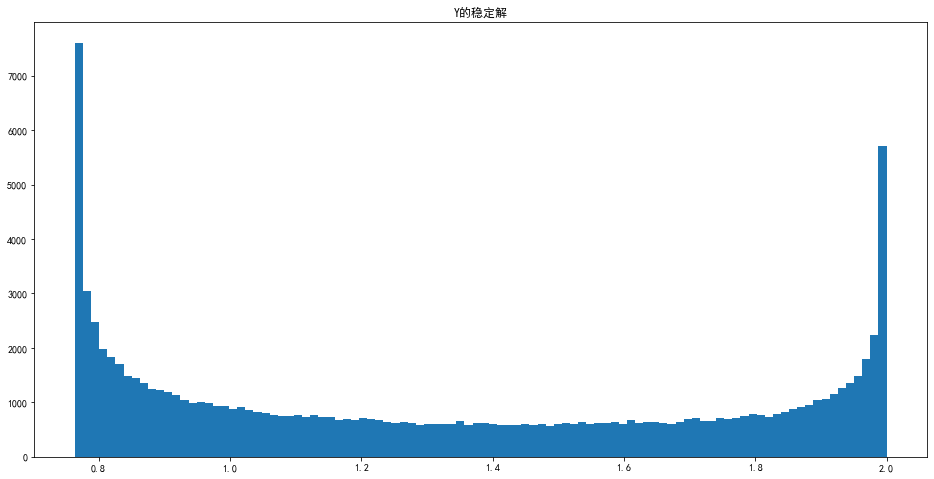
\includegraphics[width=1.95in]{images/Lotka/y.png}}
	\subfigure[Z的稳定解]{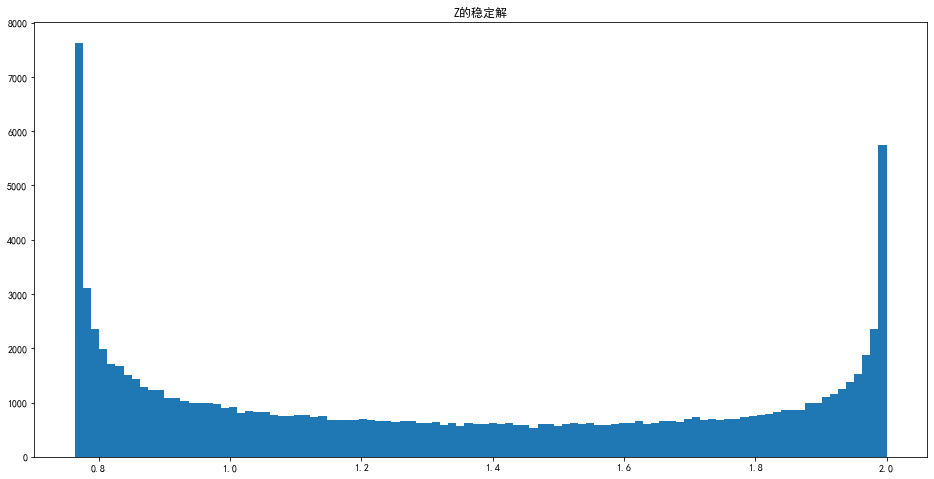
\includegraphics[width=1.95in]{images/Lotka/z.png}}
	\vspace{.2cm}
	\caption{三维随机 Lotka Volterra 方程的稳定解}
	\label{fig.6.12}
\end{figure}

















